\subsection{Bernoulli}
\paragraph{Purpose}
To estimate the outcome of an experience providing binary outcomes.
\paragraph{Theory}
\subparagraph{Parameters}
$p$ such that $\prob{X=1} = p$.
\subsection{Binomial}
\subparagraph{Purpose}
It estimates the \uB{number of successes in a sequence of $n$ independent experiments} having binary
outcomes.
\subparagraph{Parameters}
\begin{itemize}
    \item $n$: number of independent experiments
    \item $p$: probability of success, $\prob{X=1} = p$
    \item $f(k, n, p) = \prob{X=k} = \binom{n}{k}p^{k}(1-p)^{n-k}$ the probability mass function
        giving the probability to get exactly $k$ successes over $n$ independent experiments.
\end{itemize}

\begin{figure}[H]
    \begin{center}
        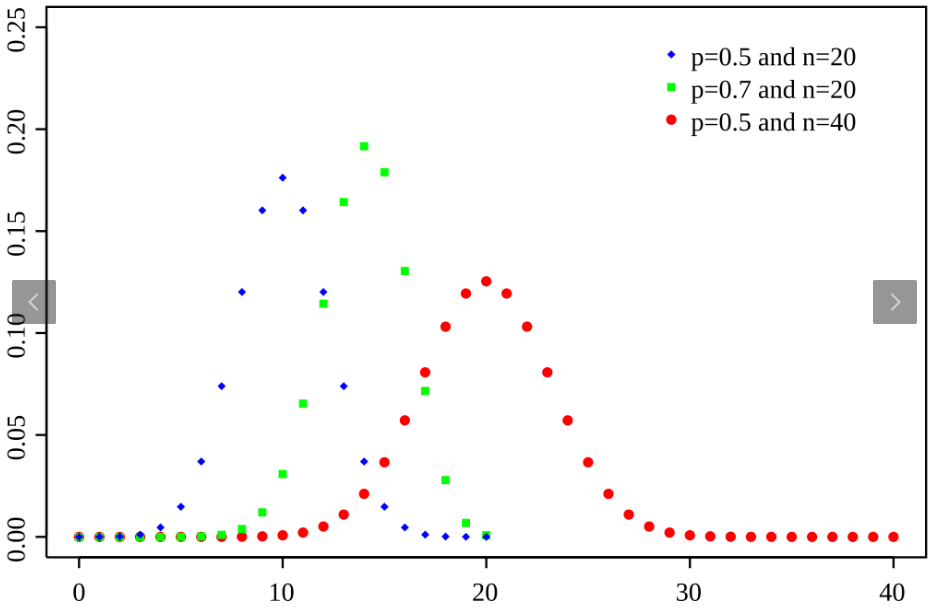
\includegraphics[width=.5\textwidth]{./chapters/2_statistics/02_common_probability_distributions/images/01_binomial_pmf.png}
    \end{center}
    \caption{Binomial probability mass function}
    \label{fig:01_binomial_pmf}
\end{figure}

\subparagraph{Approximation}
\begin{itemize}
    \item \emph{Normal distribution}: when $n$ becomes large enough the \emph{skew} gets lower and
        a reasonable approximation of $\mathcal{B}(n, p) \sim \mathcal{N}\left(np, np(1-p)\right)$
    \item \emph{Poisson distribution}: when $n\rightarrow\infty \wedge np\rightarrow C$ ($n$ should 
        be sufficiently large and $p$ sufficiently small)
        $\mathcal{B}(n, p) \sim \mathcal{P}(np)$ kn
    \item \emph{Beta distribution}: when $\alpha=k+1 \wedge \beta=n-k+1$ we have 
        $Beta(p,\alpha,\beta) = (n+1)Binomial(k, n, p)$
\end{itemize}

\subsection{Hypergeometric}
\paragraph{Purpose}
It describes the probability of $k$ successes (random draws for which an object has a given feature)
in $n$ draws \emph{without replacement} from a finite population of size $N$ that contains exactly 
$K$ objects with that feature.
\paragraph{Theory}
\subparagraph{Parameters}
\begin{itemize}
    \item $N$ (population size) $\in\mathbb{N}$
    \item $K$ (count of objects having the sought feature) $\in\inter{0}{N}$
    \item $n$ (count of draws) $\in\inter{0}{N}$
\end{itemize}
\begin{figure}[H]
    \begin{center}
        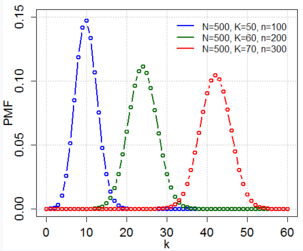
\includegraphics[width=.5\textwidth]{./chapters/2_statistics/02_common_probability_distributions/images/02_hypergeometric_pmf.png}
    \end{center}
    \caption{Hypergeometric probability mass function}
    \label{fig:02_hypergeometric_pmf}
\end{figure}

\subparagraph{Probability mass function}
$f(k; N, n, K) = \prob{X=k} = \dfrac{{K\choose k}{N-K\choose n-k}}{{N\choose n}}$

\subsection{Negative Hypergeometric}
\paragraph{Paragraph}
It describes the likelihood of $k$ successes in a sample with exactly $r$ failures.
\paragraph{Theory}
\subparagraph{Parameters}
\begin{itemize}
    \item $N$ (population size) $\in\mathbb{N}$
    \item $K$ (count of objects having the sought feature) $\in\inter{0}{N}$
    \item $r$ (count of failures) $in\inter{0}{N-K}$
\end{itemize}
\begin{figure}[H]
    \begin{center}
        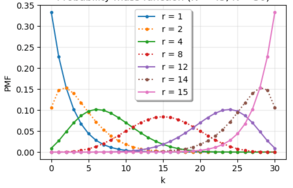
\includegraphics[width=.5\textwidth]{./chapters/2_statistics/02_common_probability_distributions/images/03_neg_hypergeometric_pmf.png}
    \end{center}
    \caption{Negative Hypergeometric probability mass function}
    \label{fig:03_neg_hypergeometric_pmf}
\end{figure}
\subparagraph{Probability mass function}
$f(k; N, r, K) = \prob{X=k} = \dfrac{{k+r-1\choose k}{N-r-k\choose K-k}}{{N\choose K}}$

\subsection{Benford's law}
\paragraph{Purpose}
It tends to describe the probability that a number, in a real-life set,  starts with a given digit
(0-9), it follows an observation that in many real-life sets of numerical data the leading digit is
likely to be small.\\
It seems that real-world distributions that span several orders of magnitude rather uniformly like
stock-market prices are likely to satisfy Benford's law very accurately, however distribution mostly
or entirely within one order of magnitude like IQ scores is unlikely to satisfy Benford's law very
accurately.
\paragraph{Theory}
\subparagraph{Parameters}
$d\in\inter{1}{9}$ the leading digit
\begin{figure}[H]
    \begin{center}
        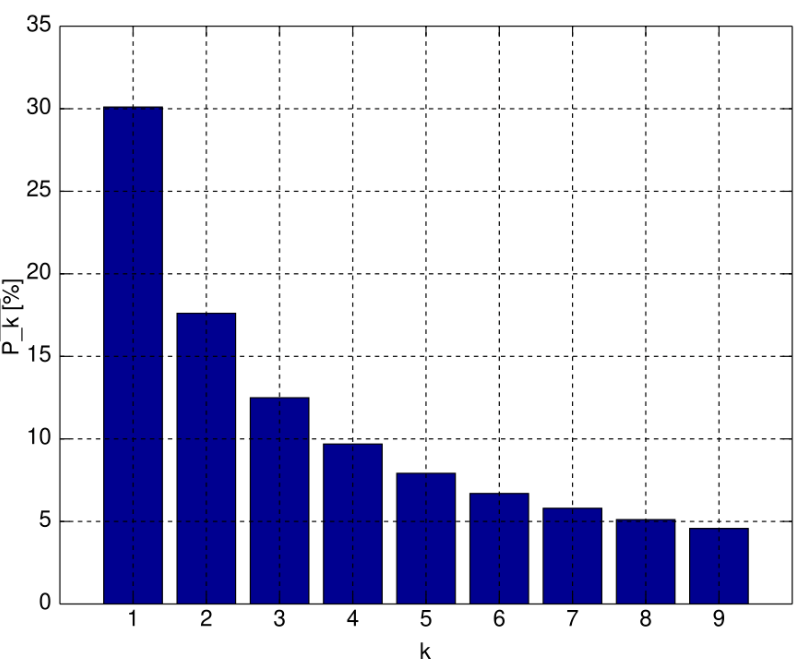
\includegraphics[width=.5\textwidth]{./chapters/2_statistics/02_common_probability_distributions/images/04_benford_law.png}
    \end{center}
    \caption{Benford's law probability density function}
    \label{fig:04_benford_law}
\end{figure}
\subparagraph{Probability mass function}
$f(d) = \prob{X=d} = \displaystyle\log_{10}(d+1) - \displaystyle\log_{10}(d) = 
\displaystyle\log_{10}(\frac{d + 1}{d}) = \displaystyle\log_{10}(1 + \frac{1}{d})$
\subsection{Zipf's law}
\paragraph{Purpose}
This empirical law states that when a list of measured values is sorted in decreasing order the value
of the n-th entry is often approximately inversely proportional to $n$.

\paragraph{Theory}
\subparagraph{Parameters}
Let's consider the generalized case where we have an inverse power law with exponent $s$ instead of 1
\begin{itemize}
    \item $s\in\mathbb{R}_{+}$ exponent of generalization
    \item $N\in\mathbb{N}_{*}$ count of elements at which we assign a rank $k$
\end{itemize}
\begin{figure}[H]
    \begin{center}
        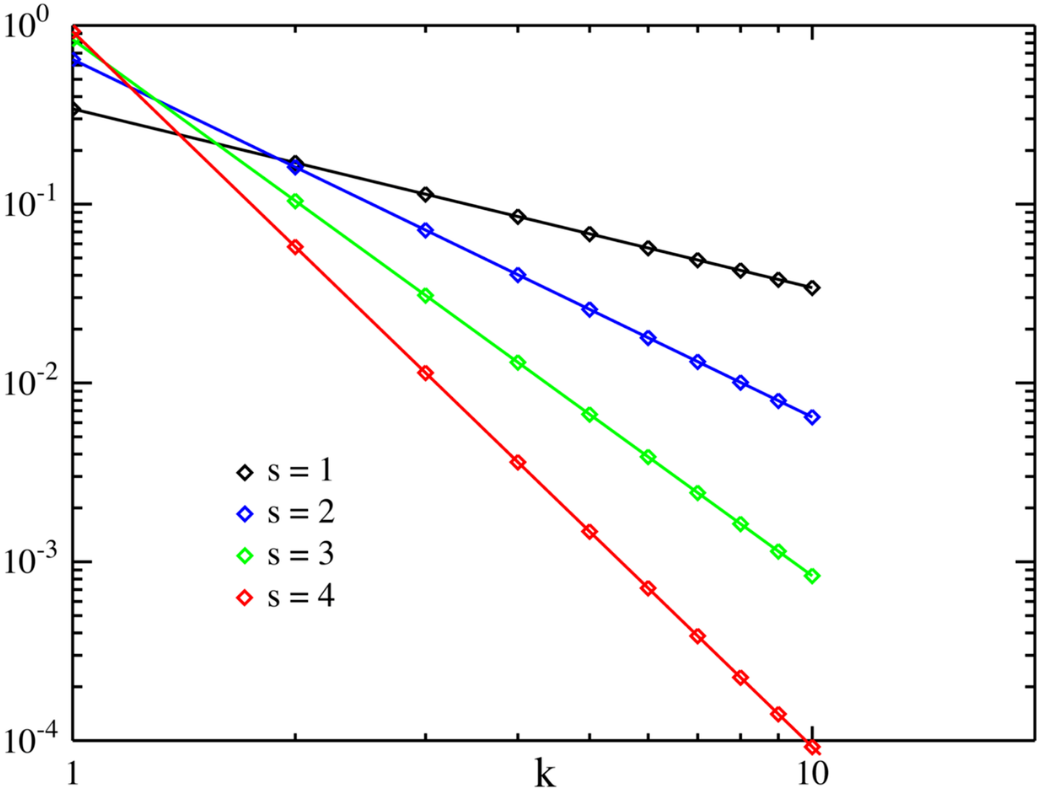
\includegraphics[width=.5\textwidth]{./chapters/2_statistics/02_common_probability_distributions/images/05_zipf_pmf.png}
    \end{center}
    \caption{Zipf's law probability mass function}
    \label{fig:05_zipf_pmf}
\end{figure}
Consider $H_{N,s} = \su{k=1}{N}\dfrac{1}{k^{s}}$ the $N$th harmonic number.\\
$f(k; N, s) = 
\begin{cases}
    \frac{1}{H_{N,s}}\times\frac{1}{k^{s}} &\Leftarrow k\in\inter{1}{N}\\
    0 &\Leftarrow (k < 1)\vee (N < k)
\end{cases}
$

\paragraph{Application}
\begin{itemize}
    \item Natural Language: $word\_frequency \propto \frac{1}{word\_rank}$
\end{itemize}

